\chapter{Trabalhos relacionados}
\label{trabalhos-relacionados}

Este capítulo apresenta alguns dos trabalhos relacionados ao tema estudado referente ao desenvolvimento de uma ferramenta para sugestão de melhorias de performance em um banco de dados.

O trabalho de \textbf{\citeonline{Chaudhuri:1997}} apresentou a proposta de simular a existência de índices em um banco de dados e utilizar o otimizador do \gls{sgbd} para estimar o custo de execução das consultas. Esse mecanismo para simulação de índices no banco de dados foi chamado de \emph{what-if} (e-se), e desde então foi utilizado em diversos outros trabalhos. Ainda, como constatado por \citeonline{Lightstone:2007}, a proposta de \citeauthoronline{Chaudhuri:1997} pode ser interpretada como o uso do otimizador do banco de dados no lugar de uma função de avaliação, utilizado em técnicas de busca em Inteligência Artificial.

No trabalho de \textbf{\citet{Alagiannis:2010}} foi desenvolvida uma ferramenta capaz de recomendar a criação de índices e particionamento de tabelas para bancos de dados PostgreSQL. A solução apresenta uma versão modificada do otimizador de consultas do PostgreSQL, adicionando um componente \emph{what-if} para simular a presença de índices e partições, além de outras ferramentas e módulos que executam isoladamente, como mostra a figura \ref{fig:arquitetura-sistema-alagiannis}.

\begin{figure}[ht]
  \centering
  \caption{Arquitetura do sistema desenvolvido no trabalho de \citeauthoronline{Alagiannis:2010}}
  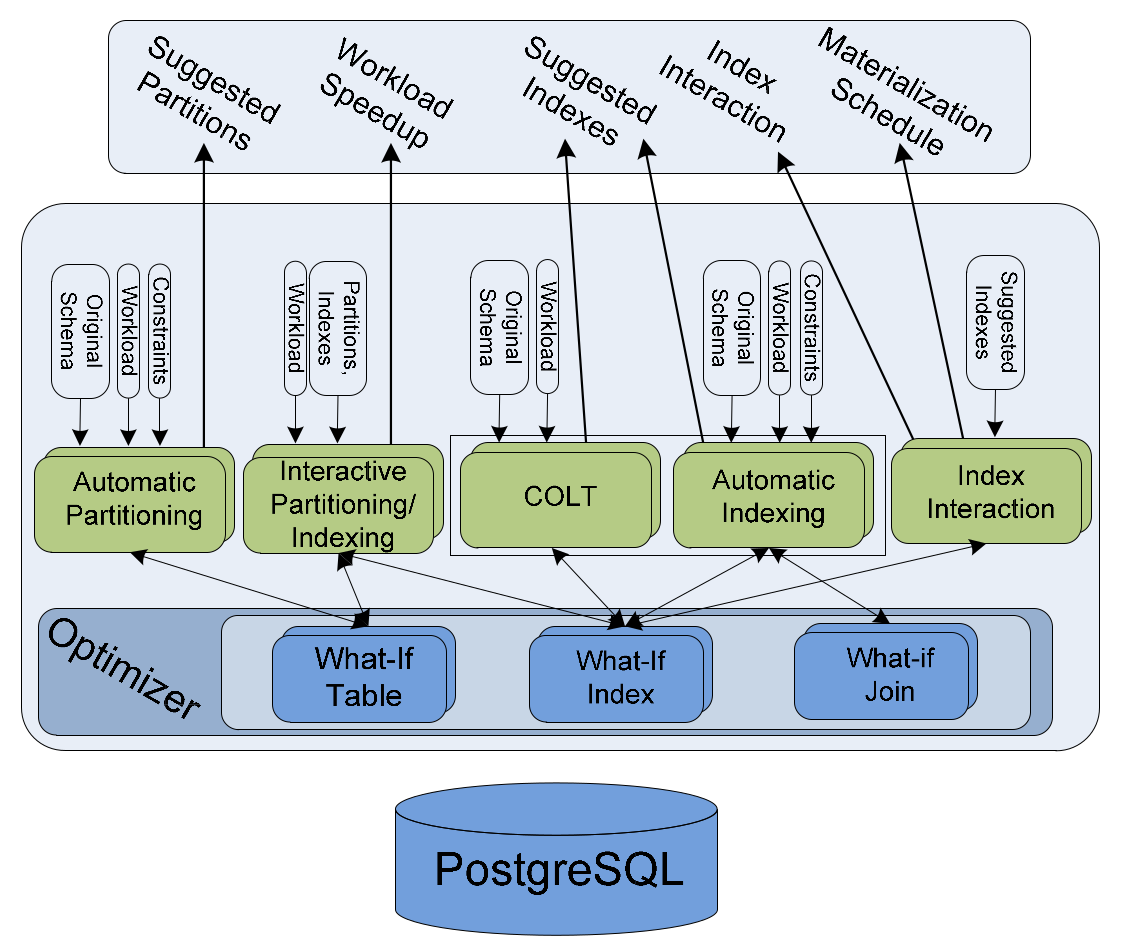
\includegraphics[width=.75\textwidth]{arquitetura-sistema-alagiannis.png}
  \fonte{\citet{Alagiannis:2010}}
  \label{fig:arquitetura-sistema-alagiannis}
\end{figure}

Para realizar recomendações de índices, a ferramenta possibilita duas alternativas: 1) sugestão automática de índices, utilizando uma abordagem \emph{offline}. A ferramenta utiliza o componente CoPhy \cite{Dash:2011} para sugerir os índices candidatos e avalia o custo das consultas utilizando o modelo INUM \cite{Papadomanolakis:2007}. A outra opção para recomendação de índices é a 2) otimização contínua, que utiliza uma abordagem \emph{online} para analisar a carga de trabalho e sugerir modificações nos índices para melhorar a performance. Esta opção é desenvolvida utilizado o \emph{framework} COLT \cite{Schnaitter:2006}, porém as alterações no banco de dados não são realizadas automaticamente, apenas é retornado um novo conjunto de índices recomendados.

O trabalho de \textbf{\citet{Agrawal:2004}} descreve a ferramenta de otimização de banco de dados integrada com o Microsoft SQL Server, o \emph{Database Tuning Advisor} (DTA), apresentada na figura \ref{fig:tela-recomendacoes-sqlserver}. As características que são suportadas por esta ferramenta para análise e recomendação de melhorias são índices, particionamento horizontal e materialização de dados.

\begin{figure}[H]
  \centering
  \caption{Interface da ferramenta \emph{Microsoft SQL Server DTA}.}
  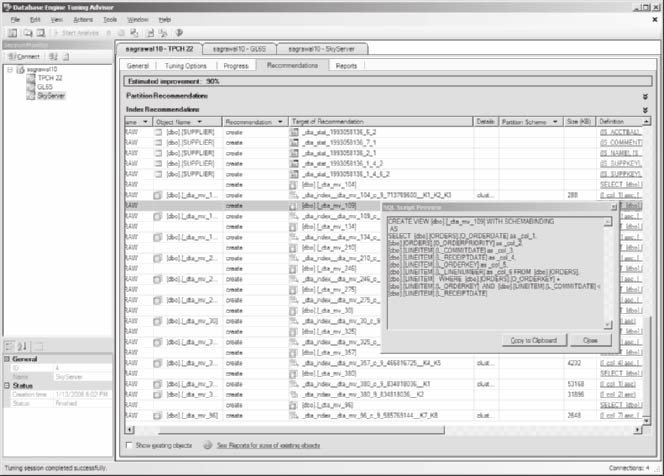
\includegraphics[width=\textwidth]{tela-recomendacoes-sqlserver.png}
  \fonte{\citet{Lightstone:2007}}
  \label{fig:tela-recomendacoes-sqlserver}
\end{figure}

Para realizar a análise e sugestão de índices, a ferramenta utiliza um componente \emph{what-if} nativo do SQL Server, desenvolvido no trabalho de \citet{Chaudhuri:1998}. A ferramenta utiliza uma interface com o otimizador de consultas do \gls{sgbd} para calcular a estimativa de custo das consultas utilizando os índices sugeridos. Os resultados dos experimentos apresentados por \citet{Agrawal:2004} mostram que as sugestões do DTA são superiores às otimizações realizadas manualmente em diferentes cenários, considerando o custo total da carga de trabalho analisada como parâmetro de comparação.

No trabalho de \textbf{\citet{Zilio:2004}} é apresentada a ferramenta \emph{DB2 Design Advisor} (figura \ref{fig:tela-recomendacoes-db2}), desenvolvida para o DB2 Universal Database (DB2 UDB), que oferece a sugestão de um modelo físico composto de índices, partições, visões materializadas e agrupamento multidimensional. O trabalho avalia duas abordagens para resolver o problema: 1) a iterativa, onde cada funcionalidade é sugerida isoladamente, porém pode ocasionar a sugestão de estruturas desnecessárias, e 2) a integrada, onde são avaliadas todas as combinações de funcionalidades e a dependência entre elas para realizar as sugestões.

\begin{figure}[H]
  \centering
  \caption{Interface da ferramenta \emph{DB2 Design Advisor}.}
  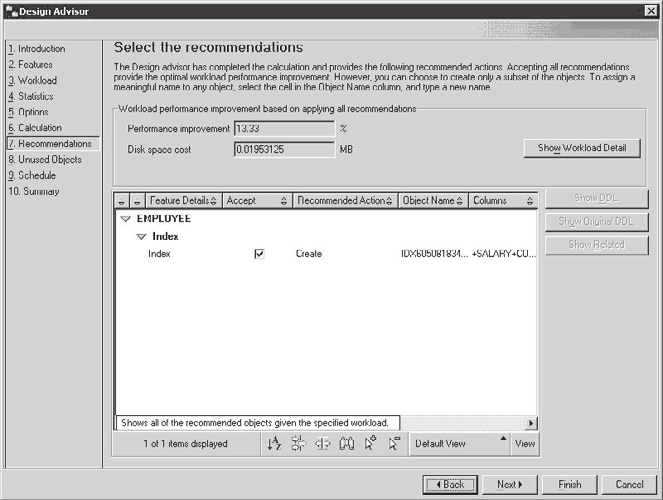
\includegraphics[width=\textwidth]{tela-recomendacoes-db2.png}
  \fonte{\citet{Lightstone:2007}}
  \label{fig:tela-recomendacoes-db2}
\end{figure}

A abordagem escolhida por \citeauthoronline{Zilio:2004} para implementar em seu trabalho foi uma abordagem híbrida, reduzindo o espaço de busca por soluções ao procurar por estruturas que dependem de outras após ter estas definidas. Para calcular a estimativa de custo das consultas foi utilizado um componente \emph{what-if} integrado ao otimizador do DB2. Ao final da execução, a ferramenta exibe uma lista de índices sugeridos e a opção para criá-los no banco de dados. Os resultados obtidos com a ferramenta representaram uma redução do tempo de execução de consultas entre 77\% e 93\% para diferentes casos. A figura \ref{fig:resultados-zilio} apresenta os resultados obtidos utilizando um banco de dados derivado de um \emph{benchmark} TPC-H\footnote{TPC Benchmark H: \url{http://www.tpc.org/tpch/default.asp}}, que consiste em um grande volume de dados e um conjunto de consultas complexas, criado especificamente para avaliações de desempenho.

\begin{figure}[H]
  \centering
  \caption{Resultados obtidos por \citeauthoronline{Zilio:2004} utilizando um banco de dados TPC-H.}
  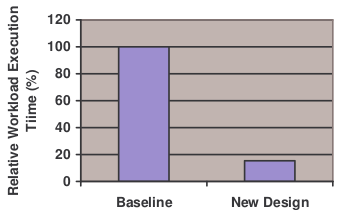
\includegraphics[width=.5\textwidth]{resultados-zilio.png}
  \fonte{\citet{Zilio:2004}}
  \label{fig:resultados-zilio}
\end{figure}

O \textbf{Percona Toolkit}\footnote{Percona Toolkit: \url{http://www.percona.com/software/mysql-tools/percona-toolkit}} é um conjunto de ferramentas para auxiliar na manutenção e administração de bancos de dados MySQL. Algumas das ferramentas relacionadas a performance são: identificação de índices duplicados e não utilizados, monitoramento de performance das operações de entrada/saída, análise de consultas lentas, verificação de configurações do \gls{sgbd}, entre várias outras ferramentas para controle de replicação e \emph{backup} \cite{PerconaToolkit:2015}.

\section{Comparativo entre trabalhos relacionados}

A tabela \ref{tab:trabalhos-relacionados} apresenta um quadro comparativo entre os trabalhos relacionados estudados, demonstrando qual o \gls{sgbd} suportado, o objetivo do trabalho, a abordagem utilizada na ferramenta e qual o modelo para avaliação do custo das consultas que foi aplicado.

\begin{table}[H]
  \centering
  \caption{Comparativo de trabalhos relacionados}
  \begin{tabular}{|p{2.1cm}|l|p{4.1cm}|p{2.1cm}|p{3.1cm}|} \hline
    \textbf{Trabalho}
        & \textbf{SGBD}
        & \textbf{Objetivo}
        & \textbf{Abordagem}
        & \textbf{Avaliação de custo}
        \\ \hline

    \citet{Alagiannis:2010}
        & PostgreSQL
        & Sugestão de índices e particionamento
        & \emph{Offline} e \emph{online}
        & Uso de componente \emph{what-if}, acessando otimizador do \gls{sgbd} para avaliar custo da consulta com \emph{cache} dos resultados
        \\ \hline
    \citet{Agrawal:2004}
        & SQL Server
        & Sugestão de índices, particionamento e materialização de dados
        & \emph{Offline}
        & Uso de componente \emph{what-if}, acessando otimizador do \gls{sgbd} para avaliar custo da consulta
        \\ \hline
    \citet{Zilio:2004}
        & DB2
        & Sugestão de índices, particionamento, materialização de dados e agrupamento multidimensional
        & \emph{Offline}
        & Uso de componente \emph{what-if}, acessando otimizador do \gls{sgbd} para avaliar custo da consulta
        \\ \hline
    Percona Toolkit
        & MySQL
        & Análise de configurações, identificação de índices duplicados e não utilizados
        & Não se aplica
        & Não se aplica
        \\ \hline
  \end{tabular}
  \label{tab:trabalhos-relacionados}
  \fonte{Elaborado pelo autor.}
\end{table}
